\documentclass[14pt,article]{scrartcl}
\usepackage[utf8]{inputenc}
\usepackage[english,russian]{babel}
\usepackage{indentfirst}
\usepackage{misccorr}
\usepackage{setspace}
\usepackage{pdfpages}
\usepackage{misc}
\renewcommand{\rmdefault}{ftm}
\usepackage[left=20mm, top=20mm, right=20mm, bottom=15mm, nohead, footskip=10mm]{geometry} % настройки полей документа
\usepackage{fancyhdr}
\usepackage{graphicx}
\graphicspath{{pic/}}
\DeclareGraphicsExtensions{.pdf,.png,.jpg}
\pagestyle{fancy}
\fancyhf{}
\fancyfoot[R]{\thepage}
\renewcommand{\headrulewidth}{0pt}
\renewcommand{\footrulewidth}{0pt}

\begin{document} % начало документа

\begin{center}
\normalsize \textbf{Федеральное государственное бюджетное образовательное учреждение
высшего образования\\
«Хакасский государственный университет им. Н.Ф. Катанова»
Институт информационных технологий и инженерного образования
Кафедра Программного обеспечения вычислительной техники и
автоматизированных систем.}\\ 
\hfill \break
\hfill \break
\hfill \break
\hfill \break
\large{РЕФЕРАТ}\\
\hfill\break
\large{по дисциплине:
«Курс информатики на английском языке»}\\
\hfill \break
\hfill \break
\hfill \break

\hfill \break
\hfill \break
\end{center}

\hfill 
\hfill \break
\hfill \break
\hfill \break
\hfill \break
\hfill \break
\hfill \break
\begin{flushright}
 Выполнил:  \\ Студент группы 36-1 \\
 Сибиреков Пётр Романович
\end{flushright}
\hfill \break
\hfill \break
\hfill \break
\hfill \break


\begin{center} \small{\bf Абакан 2017}  \end{center}
\thispagestyle{empty} % выключаем отображение  
\newpage
\tableofcontents % Вывод содержания
\newpage

\section*{Особенности Perl}
\addcontentsline{toc}{section}{Особенности Perl} 
\onehalfspacing
Общая структура Perl в общих чертах ведёт своё начало от языка Си. Perl — процедурный по своей природе, имеет переменные, выражения присваивания, блоки кода, отделяемые фигурными скобками, управляющие структуры и функции.

Perl также заимствует ряд свойств из языков программирования командных оболочек UNIX. Все переменные маркируются ведущими знаками, которые точно выражают тип данных переменной в этом контексте (например, скаляр, массив, хеш). Важно, что эти знаки позволяют переменным быть интерполированным в строках. Perl обладает множеством встроенных функций, которые обеспечивают инструментарий, часто используемый для программирования оболочки, например сортировку или вызов системных служб.

Perl заимствует массивы из Лиспа, регулярные выражения из AWK и sed, из AWK также позаимствованы хеши («ассоциативные массивы»). Регулярные выражения облегчают выполнение многих задач по парсингу, обработке текста и манипуляций с данными.

Perl 5 добавил поддержку сложных типов данных, первоклассных функций (замыкание как значение) и объектную модель. В последнюю входят ссылки, пакеты, выполнение методов от класса, переменные с лексическим объявлением области видимости, а также директивы компилятора (например, strict). Главнейшим усовершенствованием, представленным в Perl 5, стала возможность помещать код в «пакеты» (package) в качестве модулей для повторного использования. Ларри Уолл позже заметил, что «Весь замысел модульной системы Perl 5 сводился к поощрению роста культуры Perl, а не строчек кода».

Все версии Perl выполняют автоматическую типизацию данных и автоматический контроль над памятью. Интерпретатор знает тип и запросы памяти каждого объекта программы, он распределяет и освобождает память, производя подсчёт ссылок. Перевод одного типа данных в другой — например, числа в строку — происходит автоматически во время исполнения, невозможные для выполнения переводы типов данных приводят к фатальной ошибке.
\newpage

\section*{Выражения и операторы Perl}
\addcontentsline{toc}{section}{Выражения и операторы Perl} 
\onehalfspacing

Листнг кода:
\begin{verbatim}
#!/usr/bin/perl
use warnings;
$a = 3;
$b = 5;
$c = 8;
die "Старший и средний коэффициенты не должны одновременно быть нулевыми" if $a == 0 && $b == 0;
# Вычисление одного корня, если старший коэффициент равен О
$x1 = -$c/$b if $а == 0;
# Вычисление дискриминанта уравнения, если
# старший коэффициент не 0
$d = $b**2 - 4*$a*$c if $a != 0;
# Вычисление корней, если старший коэффициент
# не 0 и дискриминант положителен
($x1 = (-$b + sqrt $d)/$a/2, $x2 = (-$b - sqrt $d)/$a/2)
     unless $a == 0 || $d < 0;
# Печать результатов
print "Коэффициенты:\n a = $a b = $b с = $c";
print "\tРешение:\n\t$x1"
  if defined $x1 and not defined $x2;
print "\tРешение:\n\t$x1\t$x2"
  if defined $x1 and defined $x2;
print "\tРешения нет!" unless defined $x1;
\end{verbatim}

\hfill \break
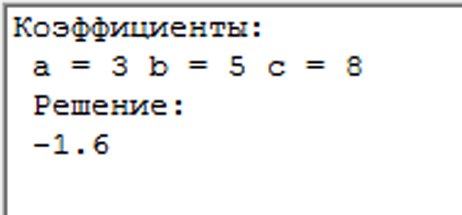
\includegraphics{q}
\end{document}  % КОНЕЦ ДОКУМЕНТА !
